% ---------------------------------------------------------------------------
% Figures (input for theory_section.tex)
% ---------------------------------------------------------------------------
\begin{figure}[t]
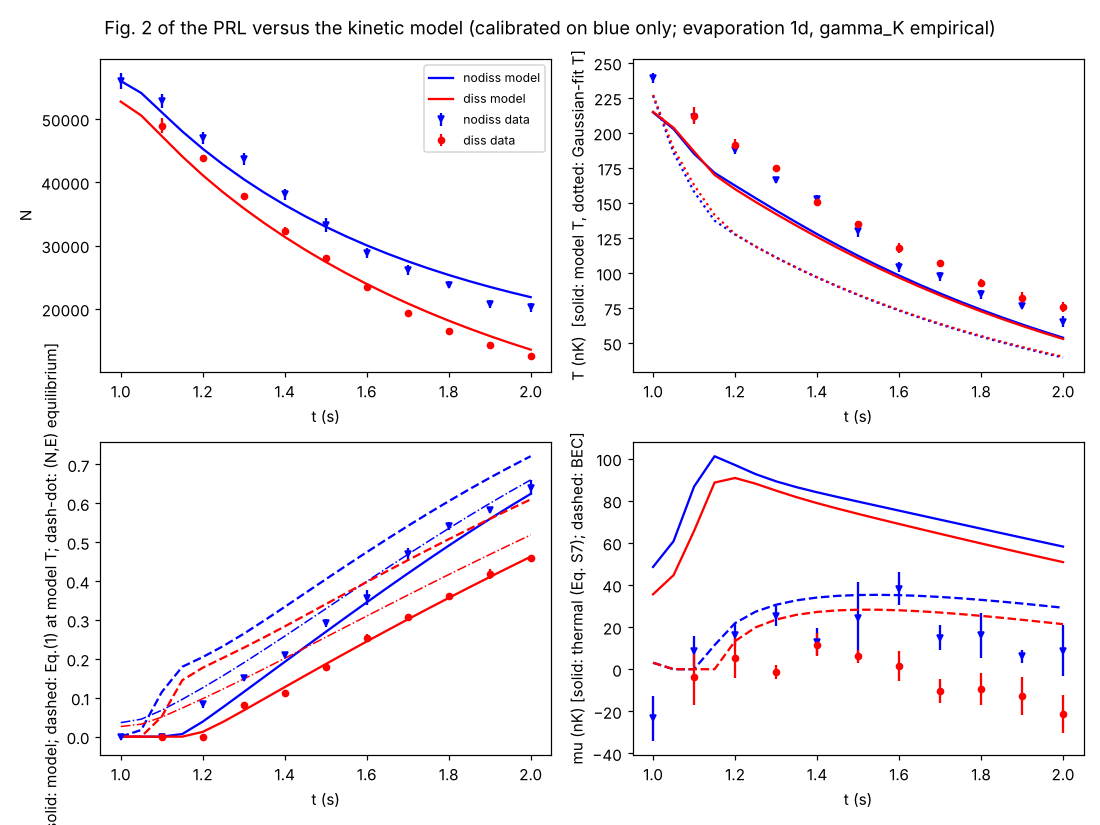
\includegraphics[width=\columnwidth]{../figures/fig2_model_1d_empirical.png}
\caption{Last second of the evaporation without (blue) and with (red) K atoms.
Symbols: data of Fig.~2 of Ref.~\cite{MelladoMunoz2020} (digitized means and
standard errors). Lines: kinetic model with $\eta_1=\etaone$, $p=\pexp$,
$\gamma_{\rm bg}=\gbg$~s$^{-1}$ fitted on the blue data only, one-direction
escape, $n=320$ energies, and $\gamma_K=0.18\,t^2$~Hz from the measured atom
numbers. (a) Total number. (b) Kinetic temperature (solid) and the temperature
a Gaussian fit to the model's momentum distribution returns (dotted). (c)
Condensed fraction (solid), Eq.~(1) of Ref.~\cite{MelladoMunoz2020} evaluated
at the model's $T$ and $N$ (dashed), and the fraction of the equilibrium at
the same $N$ and $E$ (dash-dotted). (d) Chemical potential of the thermal
cloud from Eq.~(S7) of Ref.~\cite{MelladoMunoz2020} applied to the model
(solid) and of the condensate (dashed).}
\label{fig:ramp}
\end{figure}
\begin{figure}[t]
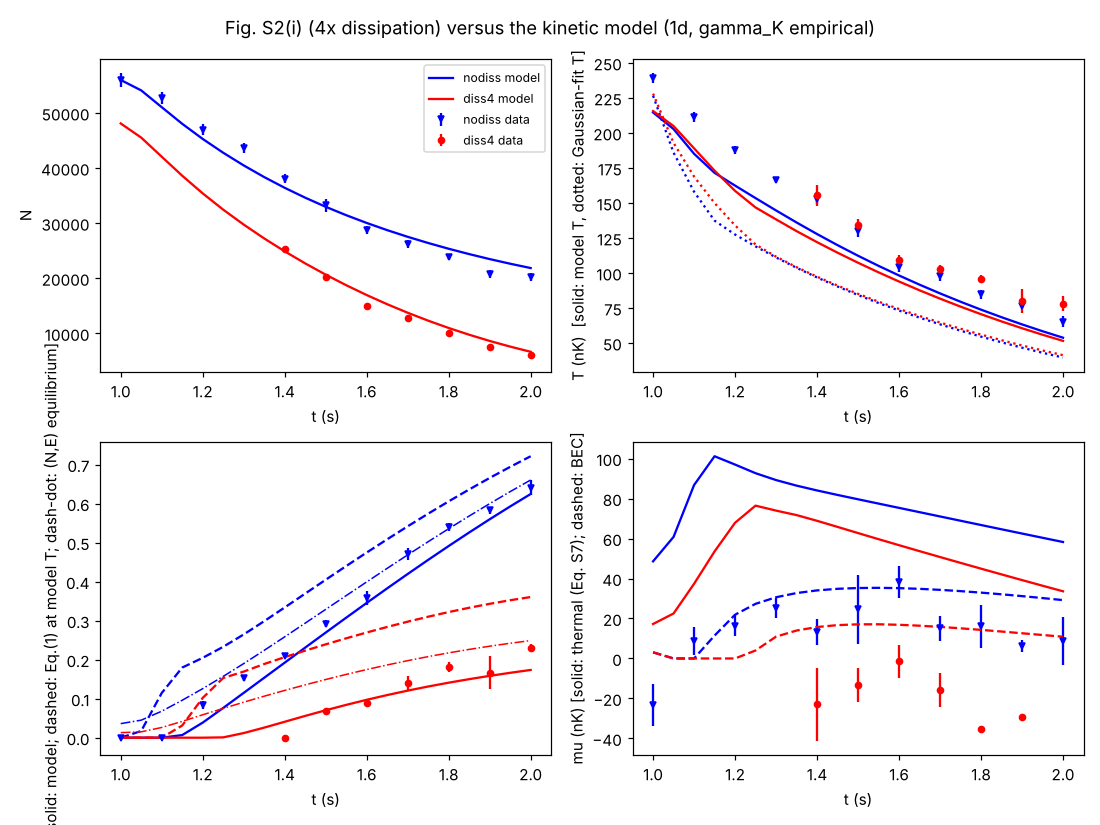
\includegraphics[width=\columnwidth]{../figures/figS2i_model_1d_empirical.png}
\caption{Same as Fig.~\ref{fig:ramp} for four times the K density
[Fig.~S2(i) of Ref.~\cite{MelladoMunoz2020}], with $\gamma_K=0.46\,t^2$~Hz.}
\label{fig:ramp4}
\end{figure}
\begin{figure}[t]
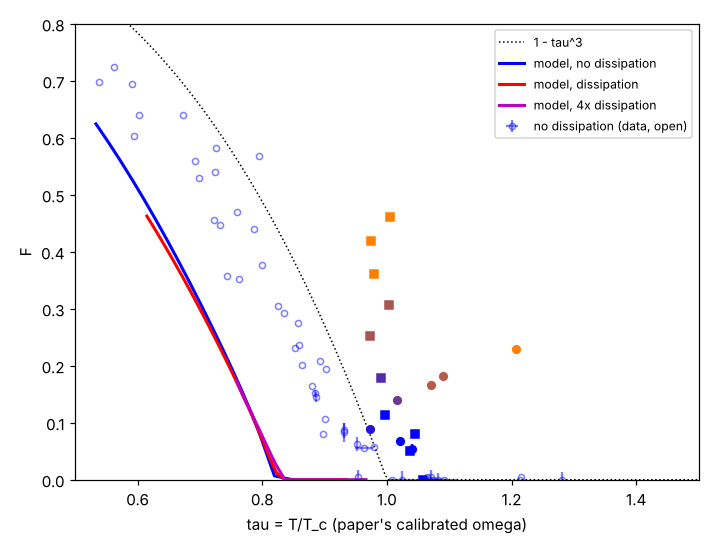
\includegraphics[width=\columnwidth]{../figures/fig3_model_1d_empirical.png}
\caption{Condensed fraction against $\tau=T/T_c$, with $T_c$ computed as in
Ref.~\cite{MelladoMunoz2020} from the calibrated frequency. Open symbols:
data without K (Fig.~3 of Ref.~\cite{MelladoMunoz2020}); filled symbols:
data with K (squares, 1$\times$; circles, 4$\times$), colour-coded in time.
Lines: model trajectories of Figs.~\ref{fig:ramp} and \ref{fig:ramp4}, using
the model's kinetic temperature. The dotted line is $1-\tau^3$.}
\label{fig:phase}
\end{figure}
\begin{figure}[t]
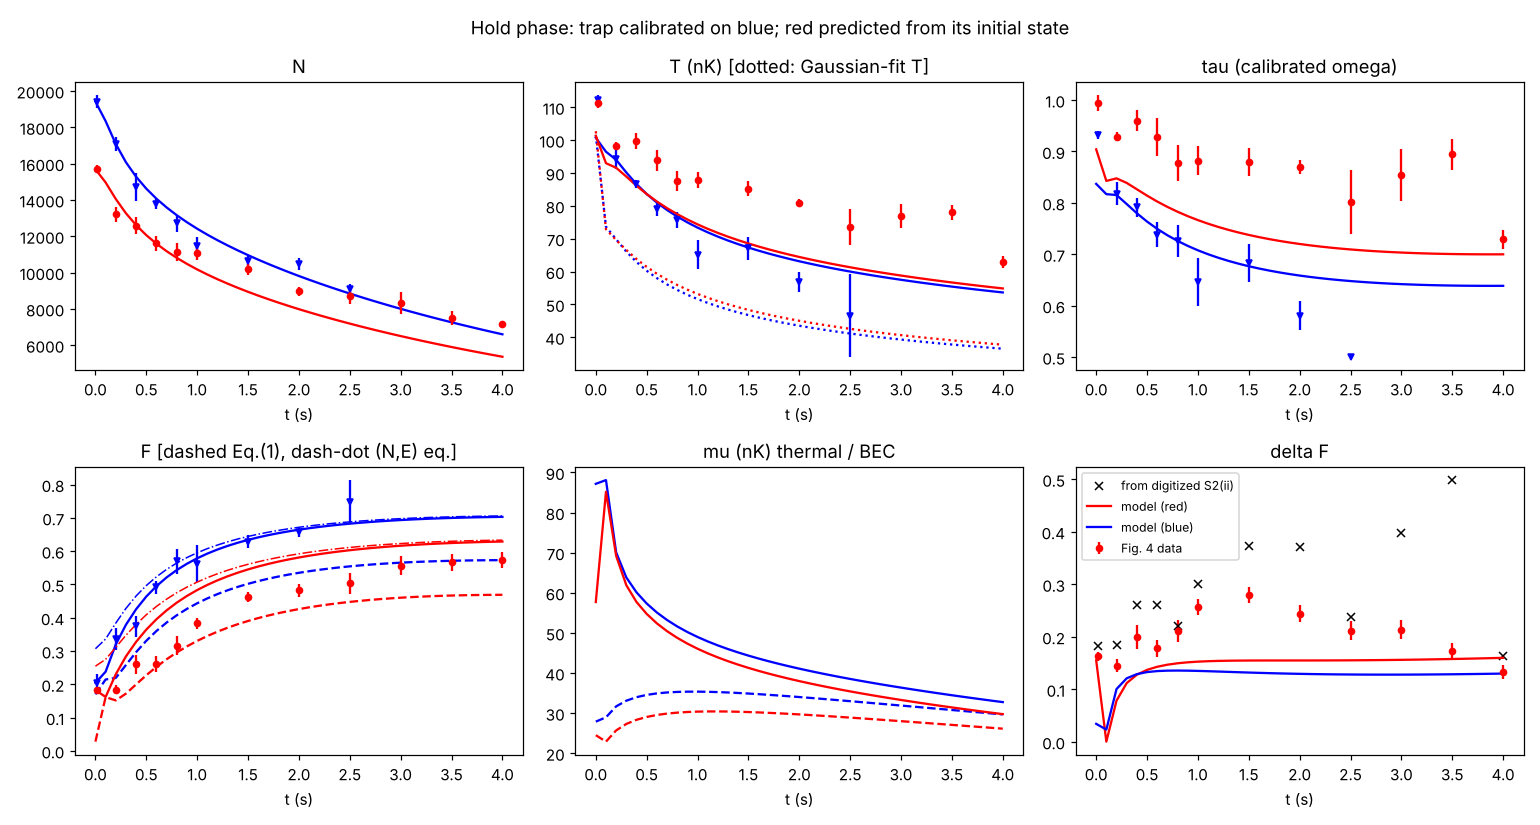
\includegraphics[width=\columnwidth]{../figures/hold_model_1d.png}
\caption{Hold at constant trap after the end of the ramp [Fig.~4 and
Fig.~S2(ii) of Ref.~\cite{MelladoMunoz2020}]. Blue: no K at any time; red: K
present before $t=0$. The trap ($\eta_{\rm hold}=\etahold$, frequency scale
$\somhold$, $\gamma_{\rm bg}=\gbghold$~s$^{-1}$) is calibrated on the blue
data; the red curves are predictions from the measured initial state. Panels
as in Fig.~\ref{fig:ramp}; the last panel shows $\delta F=F-F_{\rm eq}(\tau)$
of the model (lines), the published Fig.~4 (red circles) and the same
quantity recomputed from the digitized Fig.~S2(ii) with a constant calibrated
frequency (crosses).}
\label{fig:hold}
\end{figure}
\begin{figure}[t]
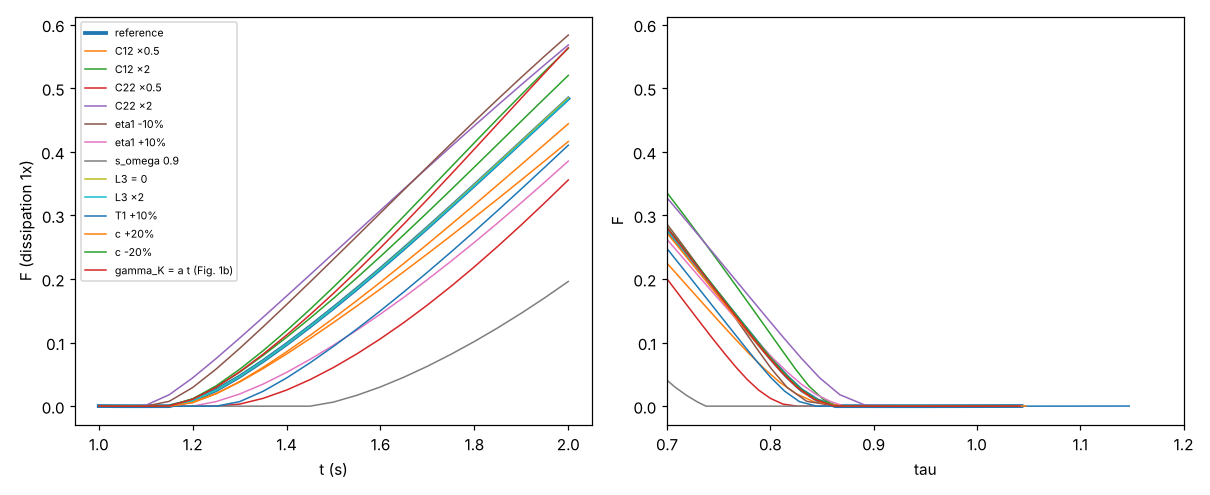
\includegraphics[width=\columnwidth]{../figures/sensitivity_1d.png}
\caption{Sensitivity of the condensed fraction with K to the model inputs
($n=240$ energies): collision integrals scaled by $0.5$ and $2$, trap depth
$\pm10\%$, frequency scale $0.9$, three-body rate $0$ and $2\times$, initial
temperature $+10\%$, loss coefficient $\pm20\%$, three-dimensional evaporation,
and the linear loss law of Fig.~1(b) of Ref.~\cite{MelladoMunoz2020}.}
\label{fig:sens}
\end{figure}
